
\def \Subject {فشرده سازی صوت}
\def \Author {رامتین احسانی }
\def \Date {1400/3/10}
\def \Session {1}
\setcounter{chapter}{\Session-1}

\chapter{\Subject}
\chapterauthor{\Author~ - \Date}

فاز اول پروژه
درس 
\CourseName 
 تهیه شده توسط
\Author
 با استفاده از سیستم حروف چینی
\grayBox {LaTeX} 
و بسته ی 
\grayBox{XePersian}


\section{فشرده سازی}
به پروسه ی encode کردن اطلاعات با استفاده از بیت های کمتر، عمل فشرده سازی گفته میشود.
در کل 2 نوع
\grayBox {Data Compression}
وجود دارد:

\begin{itemize}
    \item    
    بدون اتلاف \footnote{Lossless}
    \item
    با اتلاف \footnote{Lossy}
\end{itemize}

\begin{figure}[H]
    \centering
    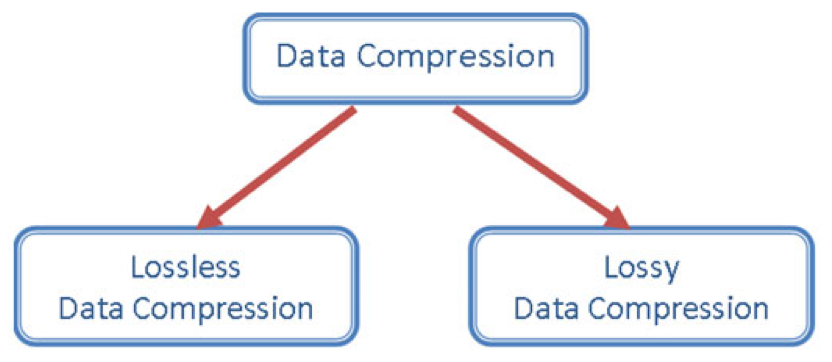
\includegraphics[width=0.5\linewidth]{images/compression.png}
    \caption{انواع فشرده سازی}
    \label{fig:mesal10}
\end{figure}
در نوع اول هیچ گونه از اطلاعات و بیت ها از دست نمیروند ولی
در فشرده سازی نوع دوم، یک سری از داده های غیرضروری و بی کاربرد را از اطلاعات داده کم میکند و تعداد بیت ها را کاهش میدهد.
انواع زیادی از داده ها را میتوان فشرده سازی کرد و در ادامه به طور مختص، فشرده سازی صوت را مورد بررسی قرار میدهم.

\subsection{اهمیت}
فشرده سازی در صنعت انتقال داده بسیار پراهمیت است.
\\
فشرده سازی باعث کاهش حجم دیتا میشود و درنتیجه میتوان تعداد فایل ها و دیتا های ثبت شده را افزایش داد و بخاطر همین باعث صرفه جویی در هزینه ها میشود.

\subsection{تاریخچه}
اولین نوع از فشرده سازی داده ها را میتوان به استفاده از مورس کد اختصاص داد که در سال 
1838 
اختراع شد. 
\\
در سال 1940 بیشتر کارهای مدرن برای فشرده سازی داده ها شروع شد و 
در سال 1951، هافمن 
\footnote{David Albert Huffman} 
الگوریتم معروف خود را معرفی کرد که از مهمترین الگوریتم های فشرده سازی داده به شمار میرود.


\section{فشرده سازی صوت}
نوعی از فشرده‌سازی داده‌است که به منظور کاهش اندازه فایل‌های صوتی طراحی شده‌است. الگوریتم‌های فشرده‌سازی صوتی در نرم‌افزارهای کامپیوتری تحت عنوان رمزگذارهای صوتی
\footnote{Audio Codec}
اجرا می‌شوند.
\subsection{فشرده سازی سوت همراه با اتلاف}
در فشرده سازی صوت همراه با اتلاف نرخ فشرده سازی بالاتری بدست می آوریم و این روش
کاربردهای زیاد و مختلقی دارد مانند:

\begin{itemize}
    \item    
    Vorbis
    \item
    MP3
    \item
    در اکثر DVD های تصویری
    \item
    کابل رادیو
    \item
    ...
\end{itemize}
در این نوع فشرده سازی، داده‌ها به ۵ تا۲۰ درصد رشته اصلی کاهش می‌یابند در مقایسه با ۵۰ تا ۶۰ درصد در بدون اتلاف.
\\
برای این نوع از فشرده سازی صوت، از راه های شناخت روح صوت
\footnote{Psychoacoustic}
برای حذف بخش های ناواضح و بی کاربرد صوت استفاده میشود. 
\\
این بخش ها به اصطلاح غیر قابل شنیدن هستند و حذف آن ها، حجم آن ها را کمتر میکند و در نتیجه به فضای کمتری برای ذخیره سازی آن ها احتیاج میشود.
\begin{figure}[H]
    \centering
    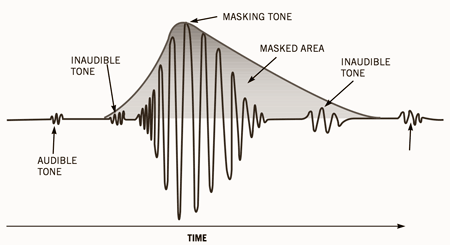
\includegraphics[width=0.5\linewidth]{images/lossy1.png}
    \caption{فشزده سازی با اتلاف}
    \label{fig:mesal1}
\end{figure}

فشرده سازی در فایل های MP3 را درنظر بگیرید.
این نوع از فایل ها بخاطر حجم کمی که دارند
بسیار بین کاربران معروف هستند و برای استفاده روزمره مناسب اند.
ولی فشرده سازی همراه با اتلاف برای افراد حرفه ای که در حوزه موسیقی کار میکنند
مناسب نیست چون داده های زیادی در این نوع از فشرده سازی از بین میرود.
\\
بنابراین همیشه کمی مصالحه 
\footnote{trade-off}
در فشرده سازی ها وحود دارد.
در صورت استفاده از فشرده سازی با اتلاف، امکان ثبت 
2 ساعت از 
فایل صوتی در 
CD
\footnote{Compact-Disk}
با حجم 
640MB
وجود دارد.
\\
ولی در صورت استفاده از بدون اتلاف،
این مقدار به 1 ساعت کاهش پیدا میکند.
\newline
\begin{figure}[H]
    \centering
    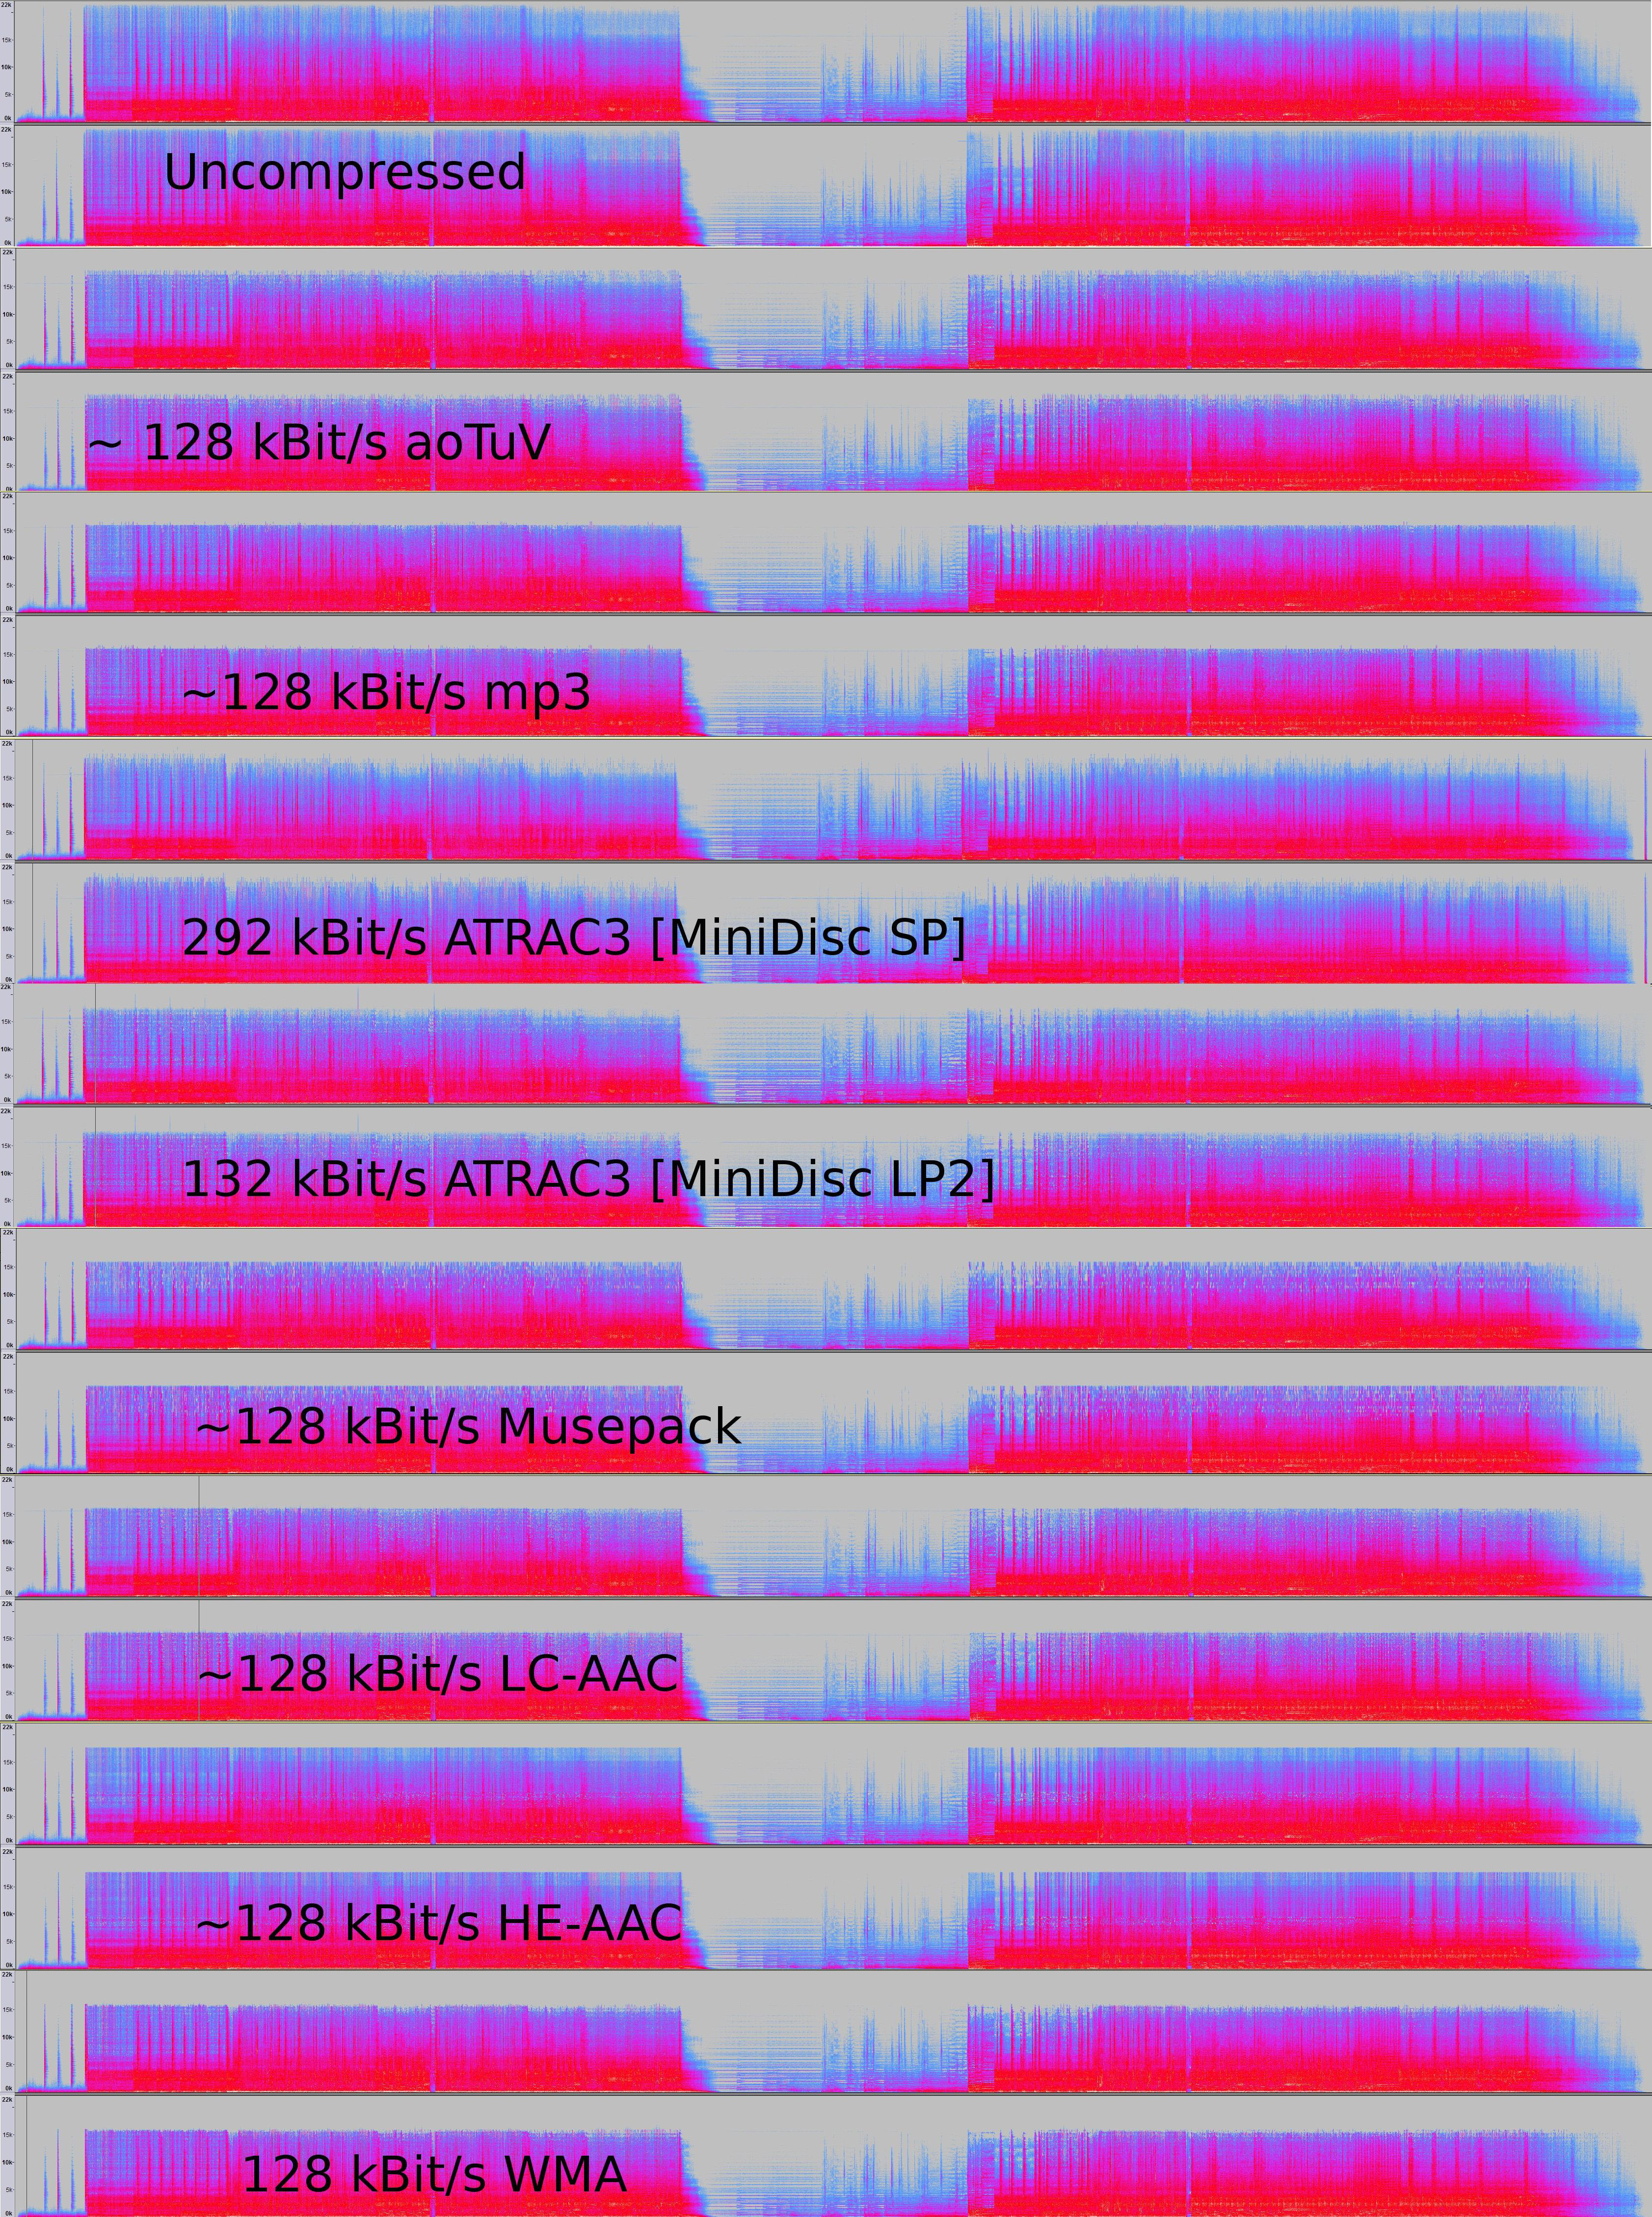
\includegraphics[width=0.4\linewidth]{images/Lossy.jpg}
    \caption{فشزده سازی با اتلاف}
    \label{fig:mesal2}
\end{figure}

\subsection{فشرده سازی صوت بدون اتلاف}
این نوع از فشرده سازی برخلاف روش قبلی، از الگوریتم هایی استفاده میکند که 
دیتای فایل صوتی فشرده شده در مقایسه با فایل اصلی، 
هیچ گونه کم و کاستی در دیتای اصلی ندارد و فقط از حجم آن کاسته شده است.
\\
هرکدام از فایل های صوتی دارای 2 بخش صداها و سکوت ها هستند.
در این روش بخش سکوت مورد هدف قرار میگیرد و فشرده سازی میشود تا این بخش ها فضایی تقریبا برابر با صفر را اشغال کنند.
\\
مثال هایی از فرمت های پر استفاده ی این روش فشرده سازی:

\begin{itemize}
    \item    
    FLAC
    \item    
    WAV
    \item   
    ALAC
    \item
    WMA Lossless
    \item
    ...
\end{itemize}
\textbf{مزایای استفاده از این روش عبارتند از:}
\begin{itemize}
    \item    
    کیفیت بالاتر
    \item    
    از دست ندادن دیتا و اطلاعات
    \item   
    قابل تبدیل به هر فرمت دیگر بخاطر از دست ندادن اطلاعات
\end{itemize}
\textbf{معایب این روش:}
\begin{itemize}
    \item    
    نرخ فشرده سازی کمتر
    \item    
    حجم بالا
    \item   
    استفاده کمتر در کارهای روزمره و ساپورت نکردن از بعضی فرمت های این روش در دستگاه های امروزی
\end{itemize}

این روش فشرده سازی برای افراد حرفه ای که در حوزه موسیقی کار میکنند بسیار مناسب است.
ولی برای استفاده روزمره و غیر حرفه ای چندان مناسب بنظر نمی آیند.
بسته به استفاده ی ما هرکدام از روش ها میتوانند برای ما مناسب واقع شوند.
\\
\begin{figure}[H]
    \centering
    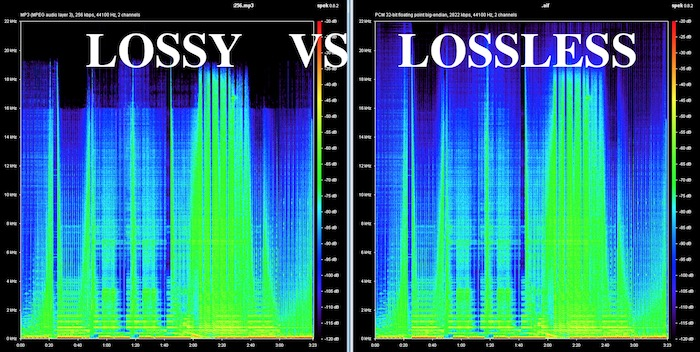
\includegraphics[width=0.5\linewidth]{images/loss-vs-less.jpg}
    \caption{مقایسه سیگنال فشرده شده در هر دو روش}
    \label{fig:mesal3}
\end{figure}
\subsection{انواع فایل های صوتی}
در ادامه تعداد بیشتری از فرمت فایل ها صوتی با روش فشرده سازی آن ها آورده شده است.
\begin{center}
 \begin{tabular}{||c c||} 
 \hline
 با اتلاف & بدون اتلاف \\ [0.5ex] 
 \hline
 \hline
 AA3 & ALAC \\ 
 \hline
 AAC & FLAC \\ 
 \hline
 MP3 & APE \\ 
 \hline
 MPC & SHN \\ 
 \hline
 OGG & TTA \\ 
 \hline
 WMA & WV \\ 
 \hline
\end{tabular}
\end{center}

\subsection{اهمیت}
فشرده سازی صوت نه تنها باعث کاهش حجم فایل میشود، بلکه باعث میشود که 
بدون دستکاری در دیتاهای فایل،
صدا بهتر و رسا تر شود .
\\
همچنین فشرده سازی باعت کاهش محدوده دینامیکی 
\footnote{Dynamic range}
- فضای بین صدای 
تیز 
\footnote{Sharp} 
و صدای 
نرم 
\footnote{Soft} 
-
میشود و صدا را دل نشین تر میکند.
\\
این موضوع در شکل 
\ref{fig:mesal4}
هم مشخص است.
\begin{figure}[H]
    \centering
    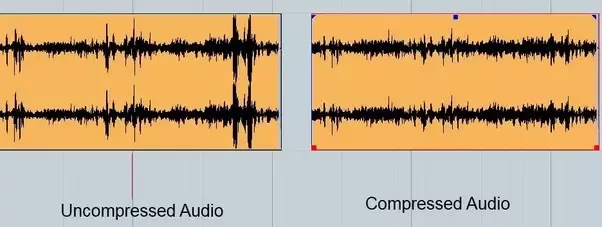
\includegraphics[width=0.5\linewidth]{images/comp-uncomp.png}
    \caption{سیگنال صوتی فشرده شده در مقابل فشرده نشده}
    \label{fig:mesal4}
\end{figure}

\subsection{الگوریتم ها}
برای فشرده سازی دیتا روش های زیادی وجود دارد که در ادامه برخی از این روش ها را توضیح میدهم.
\subsubsection{الگوریتم هافمن \footnote{Coding Huffman}}
الگوریتم هافمن از روش های فشرده سازی بدون اتلاف داده است.
این الگوریتم بر اساس ورودی که دریافت میکند درخت میکشد و بر اساس تعداد تکرار هر ورودی، به آن مقداری میدهد.
\begin{figure}[H]
    \centering
    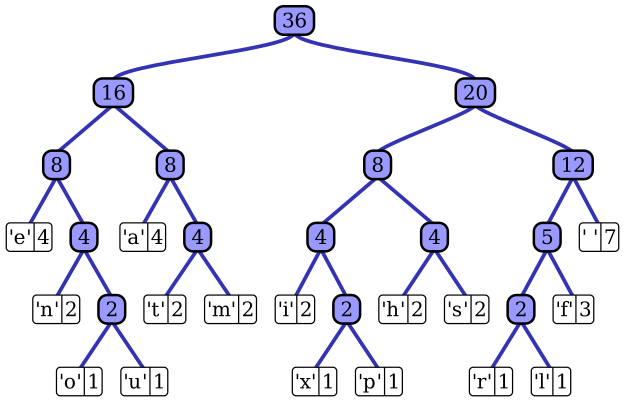
\includegraphics[width=0.5\linewidth]{images/Huffman_tree_2.png}
    \caption{نمونه درخت بدست آمده از الگوریتم}
    \label{fig:mesal40}
\end{figure}

این الگوریتم از معروف ترین الگوریتم های مورد استفاده برای فشرده سازی دیتا به خصوص صدا و تصویر است.

\subsubsection{DCT}
یکی دیگر از روش های فشرده سازی، استفاده از 
\grayBox{Discrete Cosine Transform} 
است که از فشرده سازی های با اتلاف به شمار میرود.
\\
از این روش بیشتر برای فشرده سازی تصویر استفاده میشود ولی با برای صدا هم روش مناسبی به شمار می آید.

\subsubsection{DFT}
DFT 
از تغییر دادن 
DCT 
بدست می آید و مزیتی که دارد این است که بهره وری محاسباتی بهتری دارد.
\\
استفاده از این روش فشرده سازی، بدون اتلاف است.

\subsection{\lr{MP3}}
یکی از قدیمی ترین فرمت های فشرده سازی فایل های صوتی به شمار میرود که در ادامه کمی به تاریخچه آن میپردازم.
\\
قالب ام‌پی از روی پروژه‌ای که در سال ۱۹۸۲ با مدیریت موسمن و گروهی در کنار کارل هاینز برندنبورگ در مؤسسهٔ تحقیقاتی فرانهوفر ارلانگن و دانشگاه نورنبرگ ارلانگن توسعه پیدا کرد. شرکت‌های ای‌تی‌اندتی و تامسون این پروژه را پشتیبانی کردند.
\\
در سال ۱۹۹۲ این فرمت به عنوان فرمت استاندارد صدا به‌ام‌پگ اضافه شد. اجرای این فرمت روی رایانه‌های شخصی از اوایل ۱۹۹۰ امکان‌پذیر شد.
\\
به علت نوع فشرده‌سازی امکان پخش این فرمت صدا روی خطوط دی‌اس‌ال و اینترنت نیز به راحتی امکان‌پذیر است. با ظهور نپستر و شبکه‌های پی‌توپی این فرمت خودش را بیشتر از همه گسترش داد. در سال ۱۹۹۸، امکان پخش پرتابل فایل‌های صوتی ام‌پی۳ با دستگاه‌های ام‌پی۳ پلیر ممکن شد.
\\
قالب ام‌پی۳، یک سیستم متراکم و فشرده‌سازی برای موسیقی است که باعث کاهش تعداد بایتهای موجود در یک آهنگ، به بهای اندکی افت در کیفیت صدای آن می‌شود. هدف آن فشرده‌کردن کیفیت آهنگ سی‌دی بدون از دست دادن کیفیت صدای آن می‌باشد.
\\
با یک ام‌پی۳، ۳۲ مگابایت آهنگ موجود روی یک سی‌دی به ۳ مگابایت فشرده می‌شود. اینکار باعث می‌شود که یک آهنگ را در عرض چند دقیقه بارگیری کنید و هم‌چنین می‌توانید صدها آهنگ را در سخت دیسک رایانه‌تان ذخیره کنید.
\\
این فرمت، محبوب‌ترین فرمت برای فایل‌های موزیک محسوب می‌شود. 
در واقع 
\lr{MP3} 
موفق‌ترین فرمت از خانواده ام‌پی‌ای‌جی می‌باشد.

\begin{figure}[H]
    \centering
    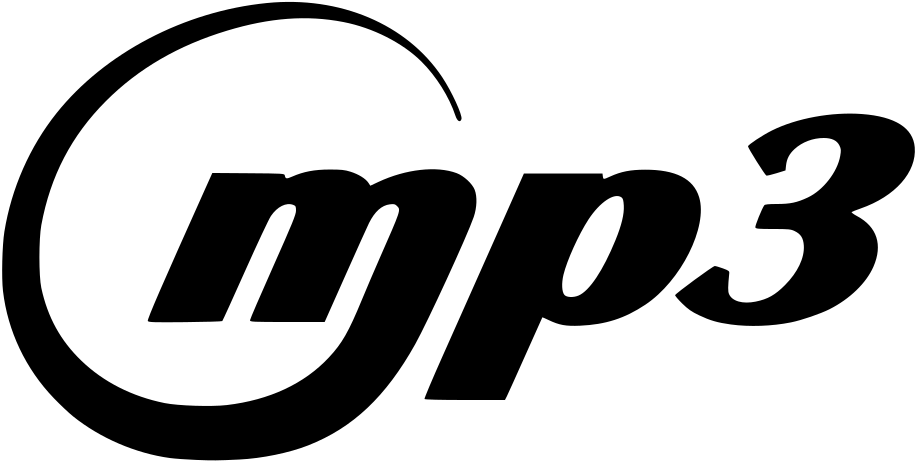
\includegraphics[width=0.5\linewidth]{images/Mp3.png}
    \caption{لوگوی معروف \lr{MP3}}
    \label{fig:mesal40}
\end{figure}

\textbf{فلوچارت فشرده سازی فایل های \lr{MP3}}
\begin{figure}[H]
    \centering
    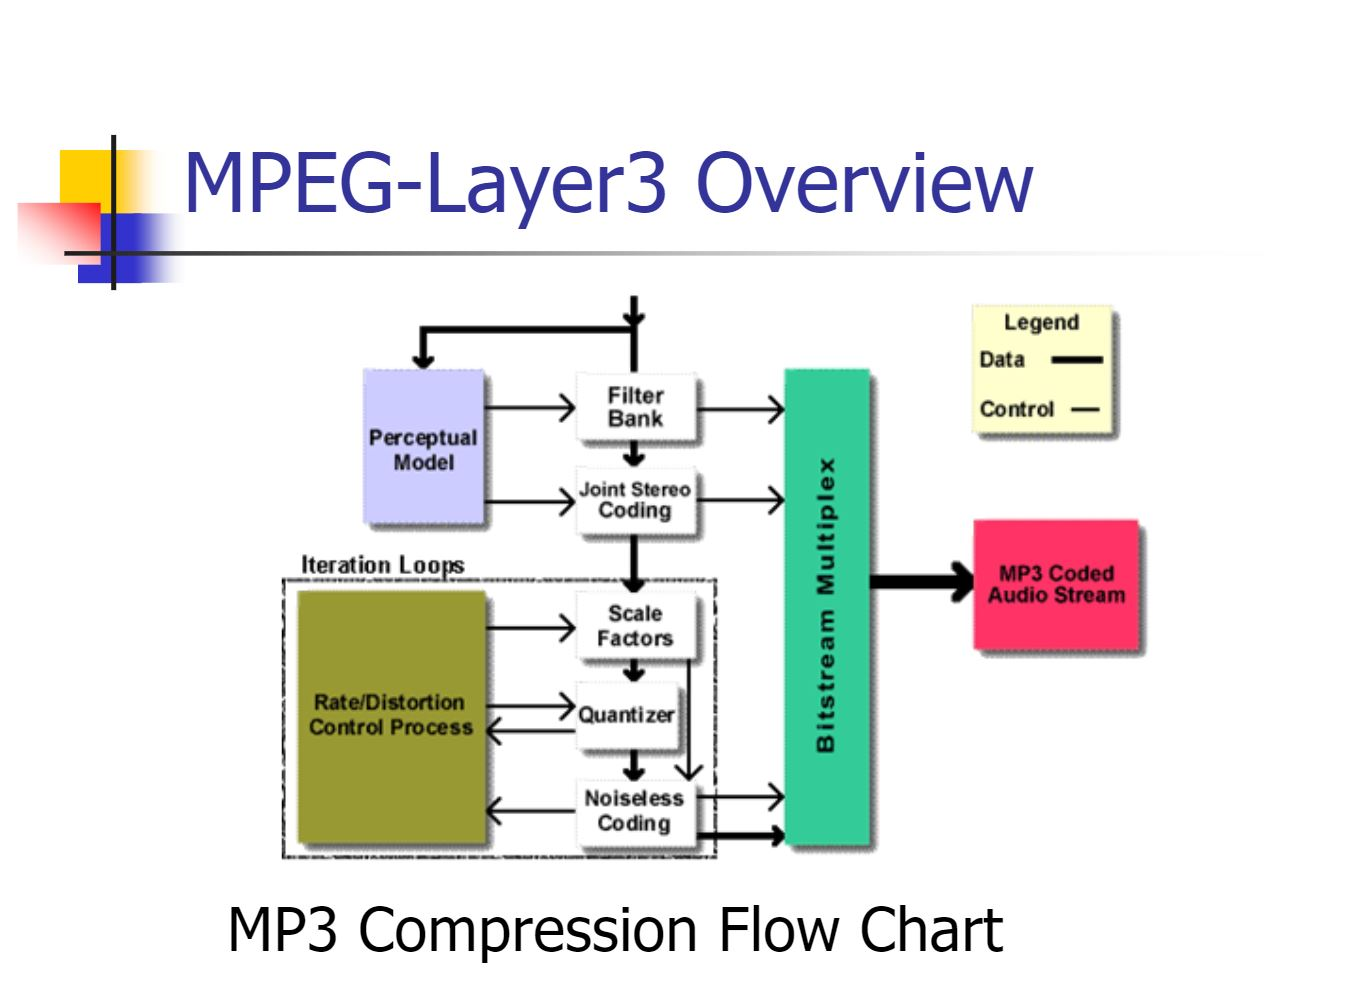
\includegraphics[width=1\linewidth]{images/mp3.JPG}
    \caption{ فلوچارت \lr{MP3}}
    \label{fig:mesal41}
\end{figure}

\section{جمع بندی}
یکی از مهمترین مبحث های انتقال داده ها، مبحث فشرده سازی است که 
روز به روز این علم جدیدتر و به روزتر شده تا بتوان به بهینه ترین شکل ممکن داده ها را فشرده کرد.
\\
در این تحقیق سعی کردم تمامی مباحث مرتبط و مهم این مبحث را جمع آوری کنم و در صفحه آخر هم منابع استفاده شده را ضمیمه کردم.
\\
در فاز بعدی با یکی از روش های آورده شده در این تحقیق، فشرده سازی صوت را با متلب پیاده سازی میکنم.
\\
\\
\\
با تشکر، رامتین احسانی
\nocite{*}
